\documentclass[12pt]{article}

\usepackage{notestyle}

\graphicspath{{./img/}}


\title{Notes Software Engineering}
\author{Brendon Mendicino}



\begin{document}

\maketitle
\newpage
\tableofcontents




\newpage
\section{Memoria}
La memoria si compone si suddivide in:
\begin{itemize}
  \item registri;
  \item cache
  \item memoria primaria;
  \item memoria secondaria;
\end{itemize}
Uno principali problemi di accesso alla memoria \`e quello di assicurarne la sua protezione, ovvero evitare che un programma in memoria riesca ad accedere alle zone di memoria di altri programmi. Una volta fatto il bootstrap, sia il SO che i programmi verranno caricati in memoria, per evitare che ogni processo abbia una vista al di fuori del suo scope, si possono usare dei controlli a livello della CPU, esistono dei registri chiamati \textbf{base} e \textbf{limit}, che attraverso dei meccanismi riescono a effettuare la protezione della memoria. Esiste anche un altro problema che \`e quello della \textbf{relocation}, che consiste nel come mappare gli indirizzi delle varie istruzioni di salto e dei vari puntatori una volta che il programma viene caricato in memoria. Se si utilizzassero degli indirizzi statici (creati solo in fase di compilazione prendendo come riferimento d'inizio del programma l'indirizzo $0$), una volta che il programma viene caricato in memoria le istruzioni punterebbero sempre allo stesso indirizzo, ma i programmi non partono tutti dall'indirizzo $0$, sorge dunque il probelema di come gestire le istruzioni che fanno riferimento ad altre parti del programma. Immagginiamo che gli indirizzi vengano creati una mentre il programma viene caricato in memoria, cosa succede se quel programma viene mosso in un altra parte della memoria? I rifermenti degli indirizzi sarabbere tutti sbagliati o addirittura potrebbero puntare a pezzi di altri programmi in esecuzione. Per questo motivo quando si utilizzano valori di indirizzi, essi vengono sommati al \textbf{base register}, mentre le boundry del programma in memoria vengono salvate nel \textbf{limit register}, grazie a questa tecnica \textbf{hardware} \`e possibile scrivere i programmi come se gli indirizzi del programma partissero da $0$.

\subsection{Indirizzamento}
Gli indirizzi vengono rappresentati in modo diverso a differenza della fase di vita di un programma: durante la compilazione vengono considerati come simbolici, durante la compilazione agli indirizzi \`e fatto il \textbf{bind} ad un indirizzo relativo (base) in modo da poter essere rilocato (questa somma \`e fatto dall'hardware), durante il linking o durante il loading. Il \textbf{binding} si pu\`o fare:
\begin{itemize}
  \item \textbf{in compilazione}: fatto quando molto semplice come nei sistemi embedded, ad esempio quando esistono solo due programmi;
  \item \textbf{in fase di load}: viene fatta la rilocazione durante il caricamento in memoria;
  \item \textbf{in esecuzione}: viene fatto il binding degli indirizzi in modo dinamico;
\end{itemize}
Per risolver questo problema ci si affida all'hardware, che \`e incaricato di fare la traduzione: l'indirizzo rimane lo stesso (logico) all'interno del processore e del programma, prima di arrivare all'address bus viene tradotto in indirizzo fisico, esiste dunque una dicotomia tra indirizzo logico e fisico, in questo modo quando si scrive un programma, l'indirizzo parte sempre da $0$. Esistono due tipi d'indirizzamento che sono di tipo logico, dove l'intervallo degli indirizzi utilizzabili \`e logico, e un indirizzamento fisico, dove il range \`e limitato dalla memoria del sistema. Per effettuare questa traduzione da indirizzo fisico a indirizzo logico e viceversa si utilizza una \textbf{MMU} (Memory Management Unit). Il modo pi\`u facile per realizzare una MMU, \`e quello di usare un \textbf{relocation register}, ovvero un registro che contiene il valore da aggiungere un indirizzo logico per fare un indirizzo fisico, il modello pi\`u semplice di MMU \`e fatto da un sommatore e un comparatore. Il \textbf{relocation register} va a sostituire il \textbf{base register}.
\begin{figure}[H]
  \centering
  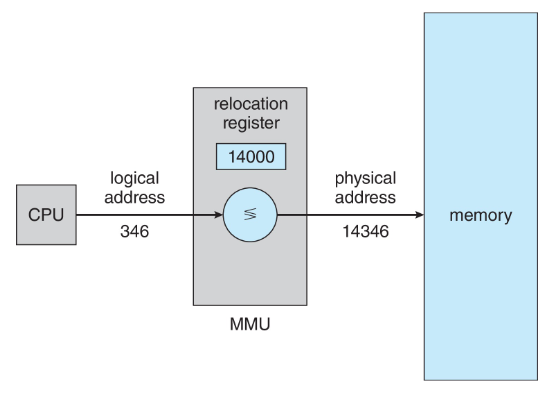
\includegraphics[width=0.6\textwidth]{basic-mmu.png}
  \caption{Basic MMU}
  \label{fig:basic-mmu}
\end{figure}
Per aumentare le prestazioni ed usare la memoria in modo pi\`u efficente si possono usare delle tecniche dinamiche.
\begin{itemize}
  \tolerance=1000
  \item Si parla di \textbf{dynamic loading} quando, un programma viene caricato in memoria principale in modo frammentato, utilizzando solo i componenti che effettivamento vengono chiamati;
  \item Si parla di \textbf{dynamic linking} quando i file che contengono le funzioni che devono essere linkate (come le librerie standard) non vengono inserite all'interno dell'eseguibile, ma gli indirizzi vengono risolti in modo dinamico durante l'esecuzione;
  \item Il \textbf{link statico} \`e quando si crea un eseguibile con tutte le funzioni dentro, di fatto il loader carica tutto quando in memoria.
\end{itemize}
Il \textbf{dynamic loading} vuol dire che una routine non \`e caricata finch\'e non \`e necessaria, questo pu\`o essere fatto quando il programmatore ne \`e consapevole, infatti il processo di load non \`e trasparente:
\begin{lstlisting}[language=c]
void myPrinf(**args) {
  static int loaded = 0;
  if (!loaded) {
    load("printf");
    loaded = 1;
  }
  printf(args);
}
\end{lstlisting}
Il \textbf{linker-assisted DL} usa una chiamata fasulla che prima chiama la load della funzione linkata dinamicamento e poi la invoca, questi piccoli pezzi di codice vengono detti \textbf{stub}.

\hfill 

Le \textbf{shared libraries} sono in grado di condividere le risorse, infatti se pi\`u processi utilizzano la stessa funzione essa viene messa a disposizione a livello globale e per ogni nuova chiamata non ci sar\`a bisogno di chiamare una load.

\subsection{Allocazione in Memoria}
\tolerance=1000
Come si alloca memoria per un programma (immagine)? La pi\`u semplice \`e l'allocazione contigua, dove si vede la RAM separata in due partizioni, una per il SO e una per i processi (indirizzi pi\`u bassi), per caricare un processo si parte da un indirizzo d'inizio e un indirizzo di fine, la MMU vista prima funziona solo con i casi di allocazione contigua (basilare). Una tecnica pi\`u efficente \`e l'\textbf{allocazione contigua con partizione variabile}, che consiste in: quando ci sono pi\`u buchi ci sono delle politiche differenti per inserire nuovi programmi:
\begin{itemize}
  \item \textbf{first-fit}: il primo che si trova;
  \item \textbf{best-fit}: il buco con la dimensione pi\`u piccola;
  \item \textbf{worst-fit}: il buco con la dimensione pi\`u grande;
\end{itemize}
La \textbf{frammentazione} \`e definita come la \emph{sparsit\`a dei buchi all'interno della memoria}. Si dice \textbf{esterna} perch\'e \`e al di fuori dei processi, si dice \textbf{interna} quando \`e interna al processo, ovvero che ha pi\`u memoria di quello che serve. La frammentazione ha bisogno di \textbf{compattazione}, il SO sposta i pezzi e poi si riparte, partiziona la memoria in zona libera e zona occupata, per fare una \textbf{deframmentazione} (o compattazione) vuol dire creare solo due partizioni (parte processi e zona libera), per effettuare la compattazione bisogna che i processi si possano spostare, inoltre un processo non pu\`o essere spostato se in quel momento sta effettuando delle operazioni di IO, una soluzione per il problema dell'IO \`e il \textbf{latch job} in cui solo la parte che sta facendo IO non pu\`o essere spostata, oppure si utilizza un \textbf{buffer IO del kernel}, si fa IO solo in buffer del sistema operativo.
\begin{definition}{Backing Store}{backing-store}
  Con \textbf{backing store} si definisce uno spazio della memoria secondaria in cui non si salvano programmi ma vengono immagazzinati dei dati che altrimenti dovrebbero andare in RAM.
\end{definition}
La \textbf{Paginazione} risolve i problemi della allocazione contigua, al suo posto si utilizzano della \textbf{pagine} che sono l'unit\`a minima di allocazione e di trasferimento, questo risolve il problema della frammentazione.
\begin{definition}{Pagine}{pagine}
  Le partizioni della memoria logica.
\end{definition}
\begin{definition}{Frame}{frame}
  Le partizioni della memoria fisica.
\end{definition}
\begin{definition}{Blocco}{blocco}
  ...
\end{definition}
Tipicamente la loro dimensione \`e un multiplo di due, sia pagine che frame hanno la stessa dimensione, da qualche parte andranno salvate le informazioni di mapping tra pagine e frame, si utilizza una \textbf{frame table}, dove ogni riga corrisponde a una mappatura. Anche utilizzando la paginazione si ha frammentazione interna. 

\hfill

Un indirizzo generato dall CPU si divide in:
\begin{itemize}
  \item \textbf{numero di pagine (p)}: 
  \item \textbf{numero di offset (d)}:
  \item \textbf{numero di frame (f)}:
\end{itemize}
Un indirizzo \`e composto da: $(p-d, d)$
\begin{example}{}{}
  Se si hanno frame piccoli diminuisce la frammentazione ma aumentano anche le righe della tabella.
\end{example}
Nelle righe della tabella si aggiungono dei bit in pi\`u per rappresentare delle informazioni aggiuntive rispetto al frame:
\begin{itemize}
  \item \textbf{parte di protezione}: specifica che la parte di codice non pu\`o essere scritta;
  \item \textbf{modify bit}: pagina modifica;
  \item \textbf{page present/absent}:  pagina presente in memoria;
\end{itemize}
\begin{figure}[H]
  \centering
  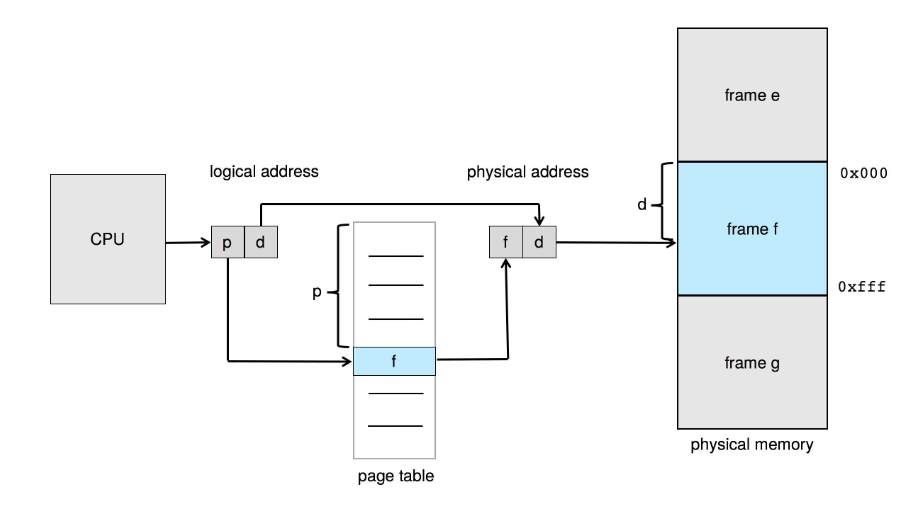
\includegraphics[width=0.7\textwidth]{page-table.png}
  \caption{Page Table}
  \label{fig:page-table}
\end{figure}
Come si implementa una \textbf{page table}? La page table si trova in memoria RAM, per sapere dove si trova si utilizzano due rigistri: \textbf{page table base register} e \textbf{base table lenght register}, infatti la base table si trova in memoria contigua. Per velocizzare questa operazione si pu\`o spostare questa tabella all'interno della CPU (le operazioni di accesso alla memoria sono costose), si usa la \textbf{Translation Look-aside Buffer} (TLB), un tipo di memoria in cui si accede per contenuto. Si aggiunge anche un altra informazione \textbf{ASID} in cui viene salvata l'infromazione del processo a cui la pagina appartiene, se non \`e presente questa informazione i processi si contendono la TLB. Quando avviene un \textbf{TLB miss} se reinserisce la pagina nella TLB e poi si ritenta, utilizzando una politica scelta. Anche usando una TLB si mantiene comunque la page table in RAM in caso di miss, in modo da recuperare il frame ed inserirlo nella TLB.
\begin{center}
  \boxed{\emph{Lo schema finale \`e la combinazione di TLB e page table.}}
\end{center}


Il \textbf{Tempo di accesso effettivo} (EAT) in memoria \`e il tempo che mi costa accedere alla RAM:
\[ EAT = h \cdot M + (1 - h) \cdot 2M  \]
\begin{itemize}
  \item $h$ = TLB hit ratio;
  \item $M$ = Memory access time;
\end{itemize}
L'accesso alla memoria \`e raddoppiato perch\'e si deve prima recupare il frame dalla page table e poi si pu\`o accedere alla memoria.
\begin{figure}[H]
  \centering
  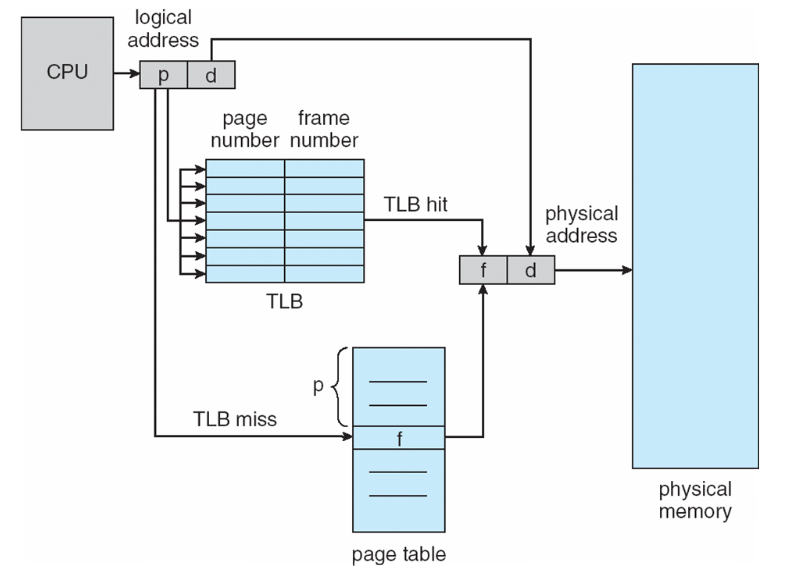
\includegraphics[width=0.7\textwidth]{paginazione-con-tlb.png}
  \caption{Paginazione Con TLB}
  \label{fig:paginazione-con-tlb}
\end{figure}
La protezione \`e implementata associando un bit di protezione per un frame specifico, e quindi per la rispettiva pagina, grazie a questo bit si possono definire parti di codice che indica che il frame \`e in solo scrittura. Anche un altro bit associato \`e il \textbf{validity} che indica quando un frame \`e valido, ovvero quando c'\`e ed \`e associata a un indirizzo in RAM, o quando non \`e valida che vuol dire che il frame non esiste o che non \`e associato ad un indirizzo, se si cerca di accedere un frame non valido viene lanciata una \textbf{trap}.

La tabella della pagina permette di \textbf{condividere le pagine} (anche se in realt\`a sono i frame), se pi\`u processi hanno delle pagine che sono comuni vengono condivise da entrambi i processi.

La page table \`e una struttura dati del kernel:
\begin{example}{}{}
  HP: spazio logico di indirizzamento di 32 bit, una pagina di 4KB ($2^{12}$), la page table avr\`a un milione di entry ($2^{32}/2^{12}$), ogni entry della page table sono 4 byte, quindi una page table \`e grande 4MB. Adesso \`e possibile avare:
  \begin{itemize}
    \item \textbf{page table contigua}:
  \end{itemize}
  Se la dimensione \`e critica (troppo grande):
    \begin{itemize}
      \item page table gerarchica;
      \item hash page table;
      \item inverted page table;
    \end{itemize}
\end{example}

\begin{wrapfigure}{R}{0.4\textwidth}
  \centering
  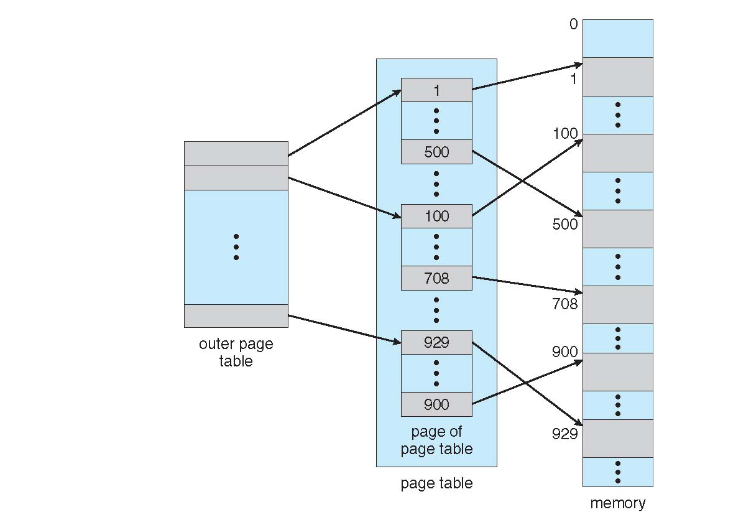
\includegraphics[width=1\linewidth]{page-table-gerarchica.png}
\end{wrapfigure}
La \textbf{la page table gerarchica}, la page table viene divisa in blocchi pi\`u piccoli non contigui, se usa una page table di livello superiore che porte alle page table di livello inferiore, questi blocchi devono rimanere contigui, anche se diventano molto piccoli. Il page number viene diviso in due parti, una per la tabella outer ed una per la tabella inner (pu\`o avere anche pi\`u di due livelli), quando si va su 64 bit e la outer dienta molto grande si pu\`o usare solo una parte dell'indirizzamento se l'eseguibili \`e molto piccolo.

\begin{wrapfigure}{L}{0.4\textwidth}
  \centering
  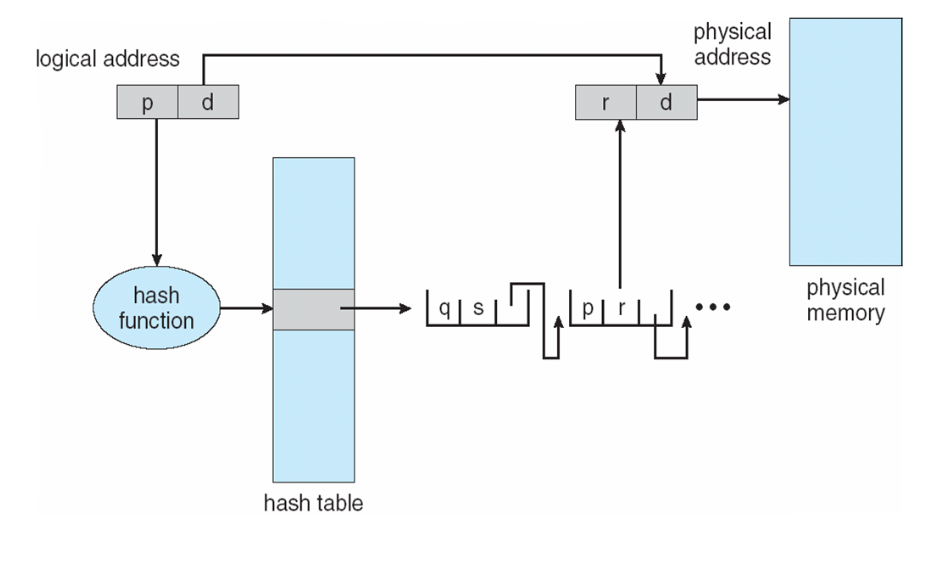
\includegraphics[width=1\linewidth]{hashed-page-table.png}
\end{wrapfigure}
La \textbf{hashed page table} permette di creare una tabella di hash, con una funzione di hash direttamente implementata in hardware che dato $p$ in input ritorna l'hash a cui \`e associato $f$. Vanno implementate delle liste di collisione, e quindi vieni immagazzinato che $p$ che \`e la chiave di accesso e come suo valore $f$. Usando una tabella di hash si potrebbe pensare anche di usare una page table condivisa tra tutti i processi, ma a quel punto andr\`a inserito l'ID del processo all'interno della chiave primaria.

\begin{wrapfigure}{R}{0.4\textwidth}
  \centering
  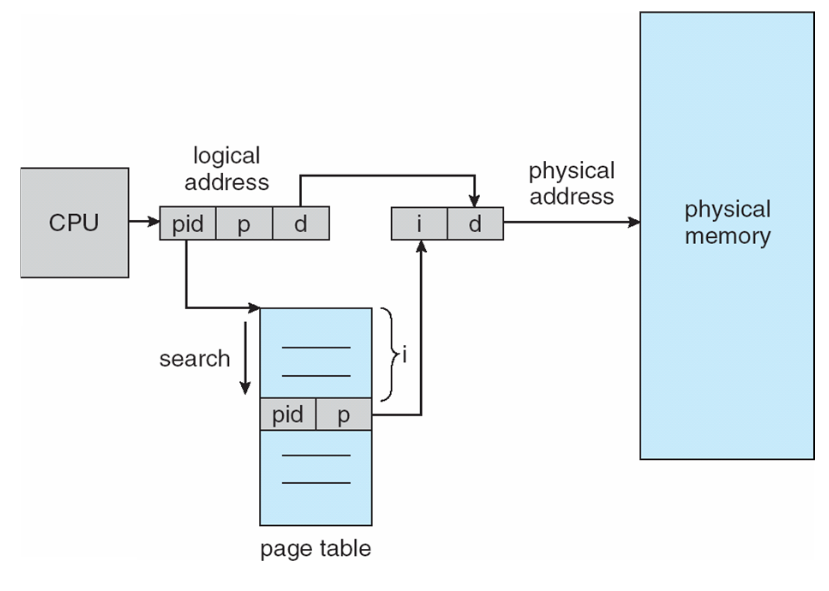
\includegraphics[width=1\linewidth]{inverted-page-table.png}
\end{wrapfigure}
La \textbf{inverted page table} \`e una tabella condivisa tra tutti i processi, la sua grandezza viene dimensionata ripetto alla grandezza della RAM e non sulla grandezza dei singoli processi, all'interno ogni frame fisico \`e associato a una pagina. In questo caso le entry che corrispondono a un frame hanno come valore di ritorno la pagina a cui \`e associato, il problema \`e che si vuole la traduzione da pagine ad entry e non il contrario, la prima strategia che si pu\`o utilizzare \`e la scansione lineare. Per rendere l'accesso pi\`u veloce viene messa una tabella di hash prima di arrivare alla tabella invertita.


\subsection{Swapping}
Si suppunga che a un certo punto si voglia far partire un processo e che la memoria sia piena, cosa si pu\`o fare? Una soluzione \`e lo \textbf{swapping}, ovvero viene la memoria associata a quel processo viene messa nel backing store (in modo temporaneo) che in linux \`e la partizione di swap, e viene caricato il nuovo processo, grazie allo swapping si possono avere processi che hanno pi\`u memoria occupata di quanto la RAM sia grande.
\begin{example}{}{}
  Quanto costa il \textbf{context switch}? Memoria piena e viene fatto partire un programma, dunque deve essere portato un processo nel backing store. 100MB da fare la swap con velocit\`a di trasferimento di 50MB/sec.
  \begin{itemize}
    \item swap out = 2000ms
    \item pi\`u swap in dello stessa grandezza
    \item il tempo totole \`e di 4s
  \end{itemize}
  Se il processo sta facendo IO non si pu\`o fare lo swap out, una soluzione \`e non spostare un processo che sta facendo IO ma spostarne un altro, oppure usare un buffer del kernel.
\end{example}
Sui telefoni non esiste lo swaping, vengono in auito le \textbf{lifecycle delle Acrivity e dei Fragment}. Il vantaggio di fare swapping \`e l'utilizzo del \textbf{paging swapping}, dove il swap in/out divento page in/out, dove vengono trasferite solo le pagine e non l'intero processo.

\subsection{Esercizi}
\begin{example}{}{}
  \begin{itemize}
    \item memoria fisica da 512MB
    \item allocazione minima 64B
    \item 128MB al SO
    \item tabella dei processi contiene: contiene indirizzo iniziale e size
    \item allocazione worst fit
    \item partizioni libere sono contenute in lista ordinata con dimensione descrescente
    \item 
  \end{itemize}
  Si supponga ...
\end{example}
\begin{example}{}{}
  Si descrivano brevemente 
  \begin{itemize}
    \item tlb: 0.9 hit ratio
    \item page table a due livelli
    \item indirizzo in tre parti, 10 11 11 bit
    \item 
  \end{itemize}
  Si fa una outer con cui si utillizzano 10bit, ed una inner con 11bit. Per calcolare il numero di inner ci sono due strade, il numero di byte preciso che contengono 100MB oppure si prende la prima potenza di 2 che contiene 100MB. Il resto delle righe delle outer overanno l'invalid bit settato ad 1.
\end{example}



\newpage
\section{Memoria Virtuale}
Con \textbf{memoria virtuale} si indica che delle pagine esistono solo virtualemente ma non fisicamente, in questo modo si vuole supportare uno spazio di indirizzamento pi\`u grande dello spazio di indirizzamento fisico. Si parte dalla premessa che \emph{un programma non bisogna di essere tutto in memoria per essere esguito}, si pensa ad un programma parzialmente caricato in memoria, dunque le mamoria di un programma non \`e pi\`u vincolato dalla grandezza della RAM, in questo caso si parla di \textbf{memoria virtuale}. Avere questa memoria virtuale porta una serie di vantaggi che volocizzano tutte le operazioni di IO tra la RAM e la memoria secondaria. La conseguenza \`e che viene introdotta la \textbf{demand paging}, ovvero che un pagina viene caricata solo quando \`e richiesta. Il \textbf{demand paging} \`e molto simile allo swapping, infatti il caso limite \`e il \textbf{lazy swapper} dove inizialmente non si ha nessun frame caricato, e ad ogni richiesta viene preso un frame.


Quasi tutto il meccansico si basa sul \emph{validity bit}, infatti l'invalid bit pu\`o rappresetnare una pagina che non ha un frame associato, i casi sono due: il frame non esiste proprio, il frame c'\`e ma deve essere recuperato, infatti il programma viene comunque caricato in memoria (backing store), perch\'e lo spazio \`e tanto.

\hfill

Il \textbf{page fault}, \`e una \emph{trap} che viene scatenata quando si cerca di accedere ad una pagina con invalid bit, il processo viene bloccato e da via al sistema operativo, i casi sono due:
\begin{itemize}
  \item \textbf{invalid refernce} $ \implies$ abort;
  \item \textbf{non in memoria}: viene recuperato il frame;
\end{itemize}
Il farme viene portato in memoria dal disco, la page table viene aggiornata, viene fatto ripartire il processo. Un caso estremo di esecuzione \`e quella di avere nessuna pagina disponibile e poi caricarle in modo incrementale.

Quanto costa una page fault?
\begin{enumerate}
  \item Trap al sistema operativo, vengono salvati tutti i registri e lo stato del processo;
  \item gestisci l'interrupt;
  \item l'OS deve verificare che quel frame esiste;
  \item recupera il frame facendo IO;
  \item quando si fa il trasferimento, l'OS viene fatto uscire dal processore e un altro processo inizia a girarare;
  \item viene tirata un eccezione al termine dell'IO;
\end{enumerate}
L'IO \`e la parte pi\`u onerosa, per calcolare l'EAT:
\begin{itemize}
  \item $p$ = probabilit\`a page fault
  \item $pfo$ = page fault overhead;
  \item $spo$ = swap page out;
  \item $spi$ = swap page in;
  \item $M$ = memory access
  \item $EAT = (1-p)\cdot M + p (pfo + spo + spi)$
\end{itemize}
\begin{example}{}{}
  \begin{itemize}
    \item memory access time = $20ns$;
    \item avg page-fault service time = $8ms$;
  \end{itemize}

  Il page fault \`e molto onerso, anche con $p$ molto piccoli i tempi sono comunque molto lenti. L'approccio migliore \`e ottimizzare il tempo del service ed ottimizzare $p$.
\end{example}


\textbf{Copy-on-write} si genera una copia di un frame solo quando uno dei processi decidono di scrivere su un frame, questo approccio viene utilizzato quando viene chiamata una \texttt{fork()}, infatti la pagine dei due processi non venogno copiate ma  sono condivise, solo quando una dei due decide di scrivere la page veien copiata ed ogni processo ha i suoi dati modificati.

\hfill

Che succede se non ci sono frame disponibili? Un processo che richiede una nuova pagina, \textbf{rimpiazza} (\textbf{page replacement}) una pagina non in uso che viene salvata sul disco, \`e possibile rimpiazzare una pagina dello stesso processo o anche di altri processi. Questa caratteristica va aggiunta nella funzione di gestione del page fault all'interno del sistema operativo, in questo caso deve essere aggiunto il \textbf{modify/dirty bit}, per gestire se delle pagine vengono modificate, se una pagina scelta ha il modify bit settato allore il frame ha un valore diverso rispetto rispetto al disco, allora primad i rimpiazzarla deve essere copiata, altrimenti \`e inutile salvare perch\'e tanto si trova gi\`a sul disco.

\textbf{Page replacement}, se non esiste un frame libero, si deve scegliere un \textbf{victim frame} da rimpiazzare, quindi oltread i tempi per portare una pagina in memoria si deve anche portare una pagina su disco. \textbf{Algoritmi di Page Replacement}:
\begin{itemize}
  \item (il processo per il momento ha un numero fisso di frame), il primo algoritmo si basa su una \textbf{string reference} che indica il numero di pagina che vengono richieste in sequenza da un processo. Viene definita la \textbf{page fault frequency}:
    \begin{definition}{Page Fault Frequency}{page-fault-frequency}
      \[ f(A,m) = \sum_{\forall w}^{} p(w) \frac{F(A,m,w)}{len(w)}  \]
      \begin{itemize}
        \item $A$ = algoritmo;
        \item $w$ = string reference;
        \item $p$ = probability;
        \item $m$ = number of availably page frames;
        \item $F$ = number of page fault generated;
      \end{itemize}
    \end{definition}
  \item \textbf{FIFO}: con 3 frames, 
  \item \textbf{Least Recently Used (LRU)}: viene ripiazzata la pagina usata per ultima. In questo caso per ogni pagina esiste un tempo associato alla pagina, questo \`e molto oneroso dal punto di vista hardware, infatti non viene adottata.
  \item \textbf{LRU algorithm}: ogni pagina ha un contatore, per ogni page fault si deve fare una ricerca del minimo. Esiste un altra implementazione a stack di numeri di pagina.
  \item \textbf{LRU Approximation Algorithm}: ogni riga ha un \textbf{reference bit}, inizialmente \`e zero e quendo si fa una reference alla pagina viene messo a 1, esiste un momento nel passato in cui i reference bit sono stati azzerati, la victim viene presa nel gruppo dei frame con reference bit a 0. \textbf{Second-chance algorithm}: si usa una fifo con reference bit, quando si incontra una pagina con 1 viene settato a 0, se si incontra uno 0 allora viene preso il victim.
  \item \textbf{Enhanced Second-Chance Algorithm}: si utilizza una combinazione di reference e modify per scegliere il frame:
    \begin{itemize}
      \item (0, 0): ...
      \item ...
    \end{itemize}
  \item \textbf{Counting Algorithm}: 
    \begin{itemize}
      \item \textbf{Least Frequently Used (LFU):}
      \item \textbf{Most Frequently Used (MFU):}
    \end{itemize}
\end{itemize}

Esercizi:
\begin{example}{}{}
    ...
\end{example}

\begin{itemize}
  \item \textbf{Page-Buffering Algorithm}: La vittima viene messa nel \emph{free pool}, ..., il SO potrebbe dare il controllo all'applicazione per la gestione della memoria.

\end{itemize}


Allocazione fissa:
\begin{itemize}
  \item si da a tutti la stessa misura (equal);
  \item si da di pi\`u a chi ha pi\`u bisogno (proporzionale): ad ogni processo si danno i frame in maniera proporzionanta.
\end{itemize}

Global vs Local allocation: un processo pu\`o scegliere una frame vittima solo tra i suoi anche tra quelli degli altri? \textbf{Locale} visto nell'esempio di sopra. \textbf{Globale}, esista una lista di free frame, si fa in modo che questa lista non arrivi mai a 0, l'idea di massima \`e che superata una soglia si iniziano a scegliere delle vittime, fino ad arrivare di nuovo ad un altra solgia, che superata permette il reinserimento dei frame.

... NUMA ...

Le prestazioni migliori si ottengono quando un processo gira su un unico processore.

Quando il sistema inizia a saturare la memoria in modo aggressivo, il SO ha due possibilit\`a: bloccare il sistema ed aspettare che un processo termini, oppure inziare a rimuovere frame, il \textbf{thrashing} \`e tenere il processore sempre attivo con dei processi.

Come si possono realizzare pochi page fault in modo statistico? Per minimizzare il numero di page fault si sfrutta il principio di localit\`a, basandosi su questo concetto si 
`e sviluppato il modello di \emph{working set} (l'insieme di pagine su cui si lavora), si definisce una finestra temporale che in cui si definisce $\Delta$ (finestra temporale e il range di pagine a cui si fanno accesso), si suppone che ci sono 10 mila accessi in memoria, $WSS_i$ (dimensione del set di pagine a cui si \`e fatto accesso, del processo $P_i$) = numero totale di pagine in cui si \`e fatto riferimento nei $\Delta$ precedenti. Ci aspettiamo:
\begin{itemize}
  \item se $\Delta$ troppo piccolo: non si riesce a contenere l'intero programma;
  \item $\Delta$ troppo grande si tengono troppe pagine in memoria;
\end{itemize}
Il \textbf{working set model}, dato un intervallo $\Delta$ si contano gli id delle pagine, se una pagina non \`e presente nell'intervallo viene rimosso dal \emph{working set}, il difetto \`e che si deve generare un'istruzione per buttare via una pagina quando esce dal working set e soprattutto si deve tenere traccia di chi deve essere buttatto fuori. Questo non si pu\`o fare in modo esatto, si usa questo principio: si tiene nel \emph{recidence set} un po pi\`u del working set, si suppongo che un timer interrompa ogni $\Delta/2$, ogni ogni pagina si tengono 2 bit di riferimento (ref bit 1, ref bit 2), uno dei due viene settato automaticamente dall'HW, ad ogni intervallo per ogni pagina a cui si fa accesso viene settato il ref bit ad 1, il ref bit che viene selezionato viene scambiato ad ogni intervallo,  quando si cambia intervallo si pu\`o decidere di rimuovere le pagine che hanno $(0, 0)$, questo approccio si pu\`o estendere con pi\`u ref bit.

Il problema del working set \`e che non guarda quante volte si fa accesso ad una pagina, si stabilisce una \textbf{frequenza di page-fault}, se il numero di page fault \`e alto allora si allarga la window, se il numero di page fault \`e basso  allora la window si restringe. Funzionamento dell'algoritmo:
\begin{itemize}
  \item si attiva l'algoritmo solo quando c'\`e un page-fault;
  \item quando si attiva si misura il tempo intercorso rispetto all'ultimo page fault $\tau$, per vedere se si sta andando bene o male;
  \item se $\tau$ \`e minore di una costante $c$ si prende un nuovo frame e lo si aggiunge al \emph{resident set};
  \item se $\tau$ \`e maggiore di $c$  si rimuove dal \emph{resident set} tutte le pagine con reference bit a zero e si settano i reference bit a zero della pagine rimanenti;
\end{itemize}
Normalmente il working set dovrebbe coincidere con i monti nel queale il SO ha delle spike di utilizzo dei frame, dovuti a vari motivi.

\hfill

Il kernel \`e allocato in modo contiguo, il motivo \`e che la maggior parte delle strutture dati presenti al suo interno sono allocate in modo contiguo, ad esempio la \textbf{page table}.

Esempio di due tipi di allocazione:
\begin{itemize}
  \item \textbf{Buddy System}: L'idea \`e che va bene l'allocazione contigua va bene ma l'allocazione pu\`o essere solo una potenza di $2$, questo causa un sacco di frammentazione interna.
  \item \textbf{Slab Allocator}: L'idea \`e allocare per pagina ma si prendono in modo contiguo. In linux c'\`e una struttura di slab allocation.
\end{itemize}


Per diminuire il numero di page fault, si pu\`o allocare un po di pagine iniziali ed essere bravi ad indovinarle, questa tecnica viene detta \textbf{prepaging}.

Quanto deve essere grande una pagina? Per diminuire la frammentazione si vorrebbere pagine piccole, per diminuire la dimensione della page table si volgiono pagine grandi. Un altro parametro \`e dato dalle operazioni di IO, infatti una volta che si legge dal disco (molto lento), tanto vale prendere tanta roba.  La grandezza prende in considerazione anche la \emph{localit\`a} dei dati. Se si guarda l'efficienza della TLB avere poche entry \`e molto meglio (pagine grandi). Solitamente le pagine hanno una grandezza compresa tra $2^{12}$ e $2^{22}$ (la grandezza \`e sempre un multiplo di $2$).

Il \textbf{TLB reach}, \`e la percentuale di spazio che la TLB vede sulla memoria (quantit\`a di memoria vista dalla TLB)
\[ TLBreach = TLBsize \cdot PageSize \]

La struttura dei programmi ha anche un effetto sui page fault.
\begin{example}{}{}
  Si supponga di voler azzerare una matrice in un doppio loop annidato.
  \begin{lstlisting}[language=c]
for (int i = 0; i < 128; i++)
  for (int j = 0; j < 128; j++)
    matrx[i][j] = 0;
  \end{lstlisting}
  \begin{lstlisting}[language=c]
for (int j = 0; j < 128; i++)
  for (int i = 0; i < 128; i++)
    matrx[i][j] = 0;
  \end{lstlisting}
  Supponendo che una riga stia all'interno di una singola pagina, il primo programma causa $128$ page faults, mentre il secondo causa $128 \times 128$ page fault.
\end{example}


\subsection{Esercizi}
Gestione della memoria 3.







\newpage
\section{OS161}
Ogni versione del kernel corrisponde ad un file di configurazione tutto in maiscolo, la prima versione \`e \texttt{DUMBVM} e tutti i file di configurzazione si trovano in \texttt{\$HOME/kern/conf}.

.....
La cartella \texttt{conf} contiene le versioni dei kernel. Per abilitare nuovi moduli si va in \texttt{conf.kern} e:
\begin{lstlisting}[language=]
defoption hello
optfile hello main/hello.c
\end{lstlisting}
\texttt{defoptions} crea un file \texttt{opt-hello.h}, che crea un file \texttt{.h} di configurazione che contiene una define per specificare se un opzione \`e abilitata o meno. Questo serve nei file del kernel per abilitare l'aggancio di altri moduli che vengono aggiunti.

Per creare compilare i nuovi moduli si pu\`o creare un nuovo file in \texttt{conf} per compilare, si pu\`o copiare uno esistene, in questo caso \`e \texttt{DUMBVM} ed aggiungere \texttt{options hello} per far compilare i nuovi file inseriti.
\begin{lstlisting}[language=c]
#if OPT_HELLO     // variabili aggiunte nei file opt-hello.h
  hello((char *)"PdS");
#endif
\end{lstlisting}

\subsection{Dumbvm e kmalloc}
L'allocazione in OS161 \`e allocazione contigua sia per i processi che per il kernel, inoltre questo allocatore non rilascia la memoria. Il file \texttt{dumbvm.c} \`e l'allocatore del mips, \texttt{vm.c} \`e un allocatore opzionale ma \`e vuoto.

\texttt{ram\_stealmem} nel file \texttt{ram.c}, perdende della pagine dalla ram e le alloca.

L'allocatore \`e diviso in allocatore User e allocatore Kernel.

Il kernel \`e basato su mips (32 bit) quindi ha 4GB di memeria logica, \`e diviso in:
\begin{itemize}
  \item \texttt{kuseg}; (0x00000000, 0x80000000) [user]
  \item \texttt{kseg0}: (0x80000000, 0xa0000000) [kernel]
  \item \texttt{kseg1}: (0xa0000000, 0xc0000000) [kernel]
  \item \texttt{kseg2}: (0xc0000000, 0xffffffff) [kernel]
\end{itemize}
Dall'indirizzo si capisce se il programma \`e kernel o user, i processi user non possono vedere lo spazio del kernel mentre il kernel pu\`o vedere lo spazio user.
\begin{figure}[H]
  \centering
  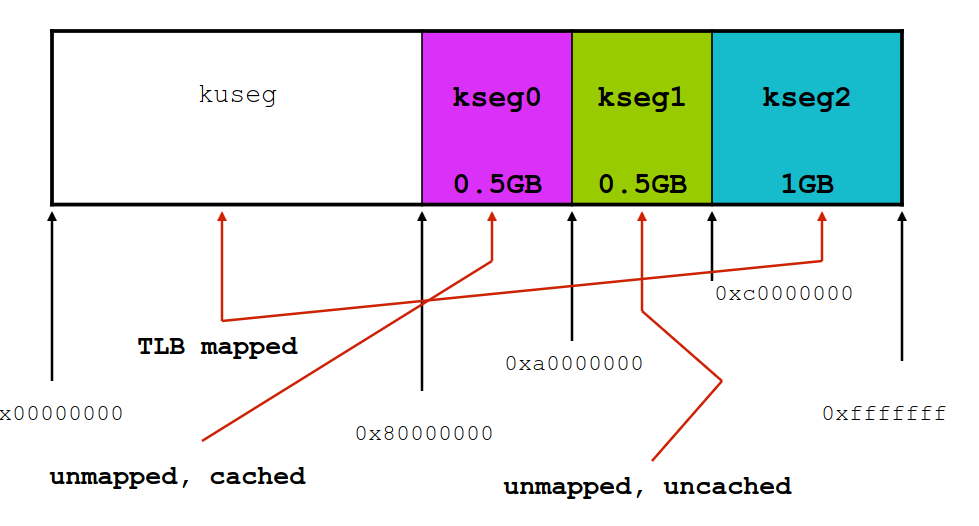
\includegraphics[width=0.8\textwidth]{mips-virtual-address-space.png}
  \caption{Mips Virtual Address Space}
  \label{fig:mips-virtual-address-space}
\end{figure}

Il kernel utilizza kseg0 e kseg1 per TLB e cache. Se si fa accesso alla memoria solo \texttt{kuseg} e \texttt{kseg2} sono mappati sulla TLB, negli altri spazi non si intende usare la TLB e quindi sono \emph{invisibili}. Il \texttt{kseg1} \`e una memoria \textbf{uncached} e patr\`a essere usata per parlare con i dispositivi di IO, il motivo \`e che questi dispositivi non funzionano bene con le cache.

Quando il kernel viene caricato la memoria \`e disposta in.
\begin{figure}[H]
  \centering
  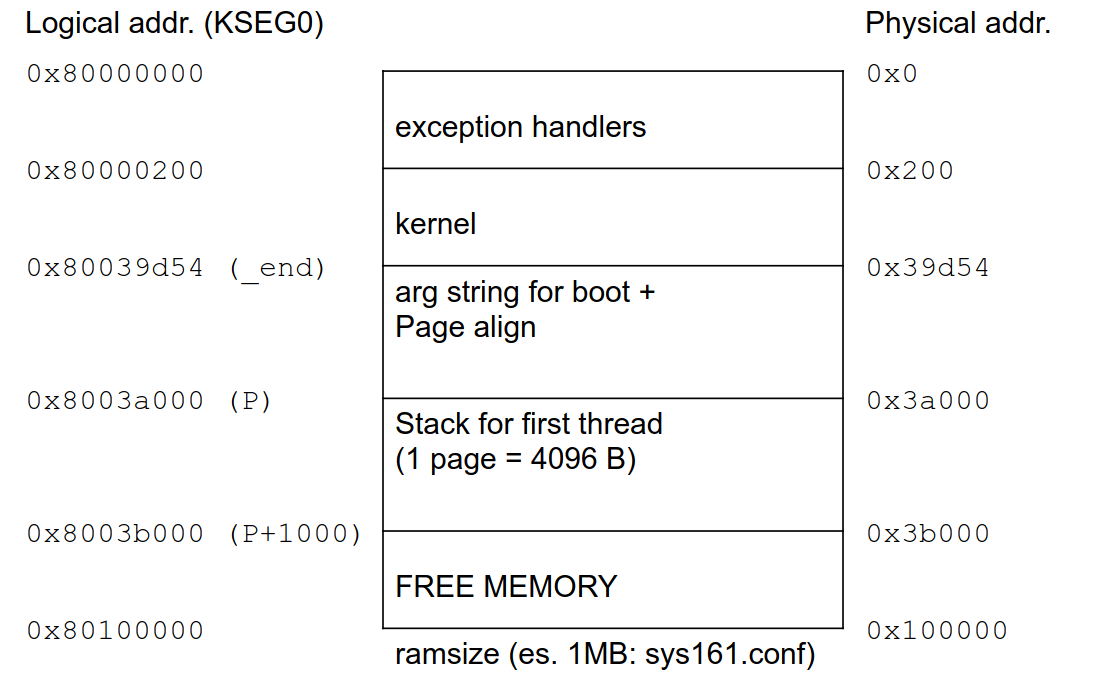
\includegraphics[width=0.8\textwidth]{kernel-loader-initial.png}
  \caption{Kernel Loader Initial}
  \label{fig:kernel-loader-initial}
\end{figure}

Una volta che viene fatto il bootstrap, si hanno a dipsosizione il \texttt{firstfree} (primo indirizzo di ram libera, logico) e \texttt{firstpfree} (primo indirizzo fisico) e \texttt{lastpaddr} (ultimo indirizzo fisico).

Quando si vuole allocare della memoria, si usa \texttt{ram\_stealmem} a cui gli vanno passete il numero di pagine.
\begin{lstlisting}[language=c]
// kern/arch/mips/vm/ram.c
paddr_t ram_stealmem(unsigned long npages) {
  paddr_t paddr;
  size_t size = npages * PAGE_SIZE;
  if (firstpaddr + size > lastpaddr) {
    return 0;
  }
  paddr = firstpaddr;
  firstpaddr += size;
  return paddr;
}
\end{lstlisting}
\begin{figure}[H]
  \centering
  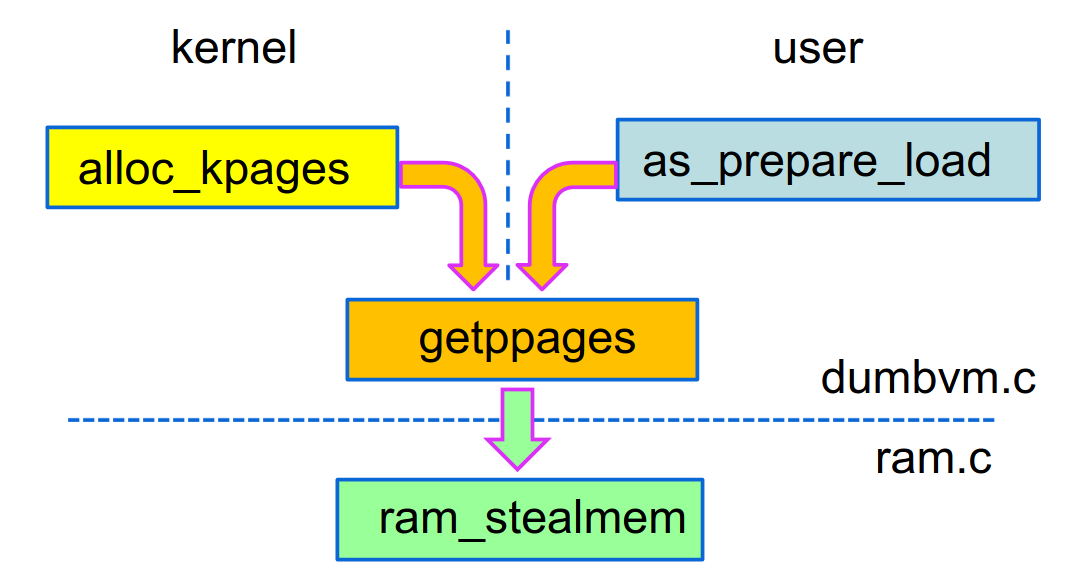
\includegraphics[width=0.7\textwidth]{interfaccia-dumbvm.png}
  \caption{Interfaccia Dumbvm}
  \label{fig:interfaccia-dumbvm}
\end{figure}
Le funzioni di free devono essere implementate.


Se si volesse gestire la paginazione, si dovrebbe scindere i l'allocatore per kernel e user, infatti l'user dovrebbe vedere delle pagine mentre il kernel della memoria contigua. Per ora la soluzione proposta \`e:
\begin{itemize}
  \item allocazione contigua (per pagine) comune;
  \item l'allocatore in bumbvm: ...
  \item bitmap implementata come char array, dove ogni posizione rappresenta se la pagina \`e libera o presa;
  \item 
\end{itemize}



\subsection{Overview}
In os161 si parla di thread di kernel e poi di processi utenti (in futuro un thread di kernel si sgancia dal kernel e diventa processo user), ogni thread ha us suo \textbf{context} di esecuzione, in cui sono contenuti dei dati e il suo stack. Gli user thread sono generati da un altro processo thread, ad esempio i \emph{POSIX pthread} permettono di creare dei nuovi thread.

La differenza tra un processo ed un thread \`e:
un processo ha uno spazio di indirizzamento in cui sono contenute le istruzioni ed i dati, poi esistono due aree che sono lo stack e lo heap, il processo arriva da un file eseguibile (tutto o in parte). Un processo pu\`o essere \emph{single-threaded} o \emph{multi-threaded}, tutti i dati globali sono condivisi e visibili dai thread, ogni thread ha privato il suo \textbf{context} (registri, stack, program counter).

In os161 il contesto di kernel thread, \`e: stack, registri, dati. I due modi di implementare la creazione dei nuovi thread \`e diviso in:
\begin{itemize}
  \item i thread sono gestiti dalla libreria;
  \item i thread sono gestiti dal kernel;
\end{itemize}
Questo \`e dovuto al fatto che: il kernl vede solo dei processi (al posto dei thread) e da come \`e fatto lo scheduler dei thread. In os161 un thread \`e fatto da:
\begin{lstlisting}[language=c]
/* see kern/include/thread.h */
struct thread {
  char *t_name; /* Name of this thread */
  const char *t_wchan_name; /* Name of wait channel, if sleeping */
  threadstate_t t_state; /* State this thread is in */
  /* Thread subsystem internal fields. */
  struct thread_machdep t_machdep;
  struct threadlistnode t_listnode;
  void *t_stack; /* Kernel-level stack */
  struct switchframe *t_context; /* Saved register context (on stack) */
  struct cpu *t_cpu; /* CPU thread runs on */
  struct proc *t_proc; /* Process thread belongs to */
  ...
};
\end{lstlisting}
Esistono 3 funzioni per gestire dei thread:
\begin{itemize}
  \item \texttt{thread\_fork}: crea un nuovo thread;
  \item \texttt{thread\_exit}: termina il thread;
  \item \texttt{thread\_yield}: sospende l'esecuzione del thread;
\end{itemize}
Quando viene creato un nuovo thread viene fatto un context switch.

Come viene fatto il context switch? Si utilizza \texttt{switchframe\_switch}, il codice scritto \`e in assembler MIPS,


Quando viene creato uno user thread, viene generato un nuovo stack per per il processo user, lo stack kernel viene comquneu mantenuto, quando il processo far\`a una chiamata ad una systema call allora passar\`a in modalit\`a kernl ed user\`a lo stack kernel che ha lasciato indietro.`













\newpage
\section{Rust}
Rust \`e un linguaggio di programmazione moderno, che non permette di avere undefined behaveiur e soprottuto \`e un linguaggio \textbf{statically strongly typed}, inlotre \`e capace di inferire i tipi di dati in modo molto potente. Rust fornisce delle \emph{astrazioni a costo nullo}, ed \`e anche \emph{interoperabile} con C. La memoria in rust \`e gestita dal programmatore solo in parte, il motivo \`e che il complilatore forza il programmatore a scrivere del codice senza errori, ed il compilatore si occupa di effettuare la gestione della memoria. Esempio di \textbf{dangling pointer} in C.
\begin{lstlisting}[language=c]
typedef struct Dummy { int a; int b; } Dummy;

void foo(void) {
  Dummy *ptr = (Dummy *)malloc(sizeof(Dummy));
  Dumyy *alias = ptr;
  ptr->a = 2048;
  free(ptr);
  alias->b = 25;  // WARNING!!
  free(alias);
}
\end{lstlisting}
Grazie alle feature di rust si possono prevenire:
\begin{itemize}
  \item \textbf{dangling pointers}
  \item \textbf{doppi rilasci}
  \item \textbf{corse critiche}
  \item \textbf{buffer overflow}
  \item \textbf{iteratori invalidi}
  \item \textbf{overflow aritmetici}
\end{itemize}
Inoltre rust propone delle convenzioni per aiutare il programmatore ad avere del codice ideomatico.

Rust parte dall'assunzoine che un valore pu\`o essere \textbf{posseduto} da una singola variabile, se la variabile esce al di fuori del suo scope il valore viene deallocato. Quando si fanno delle assegnazioni l'\textbf{ownership} del valore viene trasferito alla variabile alla quale \`e stata fatto l'assegnazione, inoltre \`e anche possibile \textbf{dare in presetito} (\textbf{borrow}) un valore; l'insieme di queste idee sono alla base della sicurezza che fornisce Rust. I puntatori sono tutti controllati in fase di compilazione, oltre all'\textbf{ownership} ogni puntatore ha un \textbf{tempo di vita} (\textbf{lifetime}), tutti gli accessi al di fuori della lifetime sono negati dal compilatore, in alcuni casi non pu\`o essere fatto l'infering della lifetime e questo andr\`a specificato esplicitamente usando la notazione \texttt{<'...>}. La \textbf{sicurezza dei thread} \`e incorporata nel sistema dei tipi e anch'essi hanno una lifetime. Rust inoltre non ha stati nascosti, come in java con le eccezioni.

I due strumenti per gestire l'ambiente di sviluppo in rust sono:
\begin{itemize}
  \item \texttt{\$ rustup}: installer and updater di rust;
  \item \texttt{\$ rustc}: compilatore;
  \item \texttt{\$ cargo}: gestione dei progetti e delle dipendenze;
\end{itemize}
I comandi di base di \texttt{cargo} sono:
\begin{itemize}
  \item \texttt{\$ cargo new project-name}
  \item \texttt{\$ cargo new --lib library-name}
  \item \texttt{\$ cargo build}
  \item \texttt{\$ cargo run}
\end{itemize}
Terminologia in rust:
\begin{itemize}
  \item \textbf{crate}: unit\`a di compilazione, crea un eseguibile o una libreria;
  \item \textbf{create root}: radice del progetto e solitamente contiene il \texttt{main.rs}, oppure \texttt{lib.rs} in caso di librerie;
  \item \textbf{module}: il progetto \`e organizzato in \emph{moduli}, se si crea un modulo come cartella il file .rs andr\`a nominato \texttt{mod.rs}, all'interno possono essere presenti moduli interni;
  \item \textbf{package}: 
\end{itemize}
Come in kotlin i blocchi condizionali hanno dei valori di ritorno. In rust non esiste l'eriditarit\`a, per\`o esistono i \textbf{trait}, che sono simili alle interfacce, offrendo la possibilit\`a di poter implementare dei metodi, ad esempio alcuni di questi sono \texttt{Display} e \texttt{Debug}, ogni tipo pu\`o implementare pi\`u tratti.

I tipi elementari di rust sono:
\begin{itemize}
  \item numerici: \texttt{i8, i16, i32, i64, i128, isize} (valore nativo del processore).
  \item numerici senza segno: \texttt{u8, ...}
  \item naturali: \texttt{f32, f64}
  \item logici: \texttt{bool}
  \item caratteri: \texttt{char} (32 bit, rappresentazione \textbf{Unicode})
  \item unit: \texttt{()} rappresenta una tupla di 0 elementi, corrisponde a \texttt{void} in C/C++
\end{itemize}
Per rappresentare le stringhe invece si use la codifica \texttt{utf-8}, che codifica i caratteri unicode in blocchi di 8 bit, la codifica utilizza la maggior parte dei primi 8 bit come caratteri standard, se si vogliono usare simboli pi\`u strani si combina un byte con il successivo, se il carattere \`e ancora pi\`u raro si utilizzano pi\`u byte, fino ad arrivare a 4. 

\hfill

Una \textbf{tupla} \`e una struttura che permette di contenere pi\`u tipi di valori, per accedere alla posizione corrispondente si utilizza la notazoine \texttt{<variabile>.<numero>}.

\hfill

Rust ha un meccanismo al suo interno per rappresentare i puntatori, infatti quando viene creato un valore in una funzione si pu\`o decidere di passare l'ownership alla funzione chiamante, che poi ha la responsabilit\`a di liberla oppure di passare ancora l'ownership, in rust esistono tre tipi di puntatori:
\begin{itemize}
  \item \textbf{reference};
  \item \textbf{box};
  \item \textbf{native pointer};
\end{itemize}
L'utilizzo dei puntatori nativi (che sono gli stessi del C), \`e possibile solo in un blocco \verb|unsafe { ... }|.

Le \textbf{reference} sono puntatori senza possesso e possono essere assegnati con \texttt{\&}:
\begin{lstlisting}[language=rust]
let r1 = &v;
let r1 = &mut v;
\end{lstlisting}
In questo caso \texttt{r1} borrows il valore \texttt{v}, per acceder al valore si utilizza la notazione per \textbf{derefenziare}: \texttt{*r1}. Quando si crea un puntatore che \texttt{\&} si pu\`o un creare un puntatore in sola lettura, si vuole anche scrivere all'indirizzo del puntatore si deve usere la keyword mut: \texttt{\&mut v}, l'accesso in scrittura \`e \emph{esclusivo}, ovvero pu\`o essere assegnato ad una sola variabile e quando viene asseganto in modo mutabile nussun altro pu\`o utilizzarlo, infatti \`e \emph{mutuamente esclusivo}.
\begin{lstlisting}[language=rust]
fn main() {
  let mut i = 32;

  let r = &i;     // r is of type "int ref";
  println!("{}", *r);

  i = i+1;        // ERROR: i was borrwed
  println!("{}", *r);
}
\end{lstlisting}
\begin{lstlisting}[language=rust]
fn main() {
  let mut i = 32;

  let r = &mut i;
  println!("{}", i);  // ERROR: i was mutably borrowed

  *r = *r+1;
  println!("{}", *r);
}
\end{lstlisting}
In questo caso la variabile \texttt{i} non \`e accessibile in alcun modo per tutta l'esistenza di \texttt{r}.

In altre situazioni c'\`e l'esigenza di allocare un dato, per prolungare la sua vita all'infuori della funzione in cui viene creato, l'equivalente della \texttt{malloc} in rust \`e \texttt{Box<T>} che alloca un parte di memoria presa dall'\emph{heap}, per creare un valore che che si vuole venga conservato, si passa a \texttt{Box} il valore che voglio si venga conservato:
\begin{lstlisting}[language=rust]
let b = Box::new(v);
\end{lstlisting}
Rust \`e in grado di fare l'infer del tipo di \texttt{v} e riesce ad allocare lo spazio necessario, quando \texttt{b} non sar\`a pi\`u visibile il \texttt{Box} verr\`a liberato dalla memoria.
\begin{lstlisting}[language=rust]
fn useBox() {
  let i = 4;                      // i si trova nello stack
  let mut b = Box::new((5, 2));   // *b si trova nell'heap, b si trova nello stack

  (*b).1 = 7;

  println!("{:?}", *b);   // (5, 7)
  println!("{:?}", b);    // (5, 7)
}
\end{lstlisting}
Quando \texttt{println!} si trova un puntatore lo dereferenzia automaticamente. Quando si arriva alla fine della funzione \texttt{a} e \texttt{b} vengono rimossi dallo stack, dato che il valore a cui puntava \texttt{b} non possiede un owner in vista quel valore viene rimosso dell'heap.
\begin{lstlisting}[language=rust]
fn makeBox(a: i32) -> Box<(i32,i32)> {
  let r = Box::new((a, 1));
  return r;
}

fn main() {
  let b = makeBox(5);
  let c = b.0 + b.1;
}
\end{lstlisting}
In questo caso il valore l'ownership del valore puntato da \texttt{r} passa la sua ownership a \texttt{b} che si trova nel \texttt{main}, quando il \texttt{main} termina e la vita di \texttt{b} finise il valore puntato viene anch'esso liberato.

I \textbf{Puntatori nativi} sono \texttt{*const T} e \texttt{*mut T}, il \texttt{*} indica un puntatore nativo e possono essere utilizzati solo nei blocchi \texttt{unsafe { ... }}.

Rust supporta nativamente anche gli \textbf{array}, in rust gli array sono composti da dati omogenei allocati contiguamente nello stack. Si possono inizializzare nel seguente modo:
\begin{lstlisting}[language=rust]
let a: [i32; 5] = [1, 2, 3, 4, 5];
let b = [0; 5];     // array lungo 5, inizializzato a 0
\end{lstlisting}
In rust gli array hanno la conoscenza di quanto sono lunghi. Se si cerca di accedere ad indice fouri dal range di utilizzo rust fa \texttt{panic}, se \texttt{panic} viene lanciato in nel thread principale il programma termina, se viene lanciato in un altro thread viene terminato il thread. Per accedere all'array si utilizzano gli \textbf{Slice} (invece di utilizzare i puntatori), che vengono creati come riferimento ad una porzione di un array:
\begin{lstlisting}[language=rust]
let a = [1, 2, 3, 4];
let s1: &[i32]  = &a; // s1 contiene 1, 2, 3, 4
let s2 = &a[0..2]     // s2 contiene 1, 2
let s3 = &a[2..]      // s3 contitne 3, 4
\end{lstlisting}
Per questa sua natura viene detto \textbf{fat pointer}, perch\`e oltre a contenere il puntatore contiene anche la lunghezza. Come nel caso degli array se si va al di fuori del range viene generato un \texttt{panic}.

Il problema degli array \`e che quando vengono creati con una dimensione, questa rimane fino alla del loro lifetime, un array variabile pu\`o essere creato con \texttt{Vec<T>} che rappresenta una sequenza di oggetti di tipo \texttt{T}, al contrario degli array gli oggetti presenti in \texttt{Vec} sono allocati nell'heap.
\begin{lstlisting}[language=rust]
fn useVec() {
  let mut v: Vec<i32> = Vec::new();

  v.push(2);
  v.push(4);

  let s = &mut v;
  s[1] = 8;
}
\end{lstlisting}
Quando viene inizializzato \texttt{Vec} nello stack vengono inseriti 3 parametri: pointer, size, capacity. Appena viene fatto push viene allocata della memoria nell'heap, e i parametri size e capacity vengono aggiornati. Se vuole creare uno slice \texttt{s}, nello stack viene messo un fat pointer, ovvere il puntatore all'heap ed il size corrente. Quando \texttt{Vec<T>} viene inizialmente inizializzato, nel campo puntatore viene inserito l'allinemento che il tipo \texttt{T} dovr\`a avere in memoria.

Lo stesso discorso fatto per i \texttt{Vec} vale per gli oggetti di tipo \texttt{String}. Quando si crea una stringa tra le virgolette viene creato un \texttt{\&str} e non una \texttt{String}, questo dato andr\`a inserito nella sezione del programma dei \emph{dati inizializzati}, al contrario delle \texttt{String} queste non modificabili, se si vuole utilizzare una stringa si utilizza \texttt{"...".as\_str()}, che ritorna uan stringa allocata nell'heap.
\begin{lstlisting}[language=rust]
fn main() {
  let hello: &str = "hello";

  let mut s = String::new();    // il valore (futuro) puntato da s viene allocato nell'heap

  s.push_str(hello);            // l'heap viene inizializzato una capacita' ed un size uguale al size della stringa puntata da "hello"
  s.push_str(" world!");
}
\end{lstlisting}
In rust le keyword \texttt{let} e \texttt{let mut} sono delle istruzioni, mentre un blocco racchiuso tra \texttt{{ ... }} \`e un espressione e quindi ha un valore di ritorno, anche il costrutto \texttt{if} \`e un espressione, \textbf{il valore viene ritornato a patto che l'ultima istruzione del blocco non abbia un punto e virgola}. Si pu\`o asseganre un etichetta con \texttt{'<nome-etichetta>:} ad un espressione per poter specificare il ritorno:
\begin{lstlisting}[language=rust]
fn main() {
  'outer: loop {
    'inner: loop {
      //...
      continue 'outer;
    }
  }
}
\end{lstlisting}

Per leggere gli argomenti passati da linea di comando si utilizza:
\begin{lstlisting}[language=rust]
fn main() {
  let args: Vec<String> = args().skip(1).collect();

}
\end{lstlisting}
Si pu\`o utilizzare la libreria \texttt{clap} per fare il parsing degli argomenti. per farlo si pu\`o andare nel file \texttt{.toml} ed inserire la dipendenza.


Per fare IO da console si utilizza \texttt{stdin}:
\begin{lstlisting}[language=rust]
fn main() {
  let mut s = String::new();

  if io::stdin().read_line(&mut s).is_ok() {
    println!(..., s.trim());
  } else {
    println!("Failed!");
  }

  // Oppure...
  io::stdin().read_line(&mut s).unwrap();
  println!(..., s.trim());
}
\end{lstlisting}


\subsection{Ownership}
Il concetto dell'ownership in rust permette al \textbf{borrow checker} di controllare l'utilizzo corretto dei puntatori, in rust \emph{un valore pu\`o essere posseduto da una e una sola variabile}, il fallimento di questa condizione comporta ad un fallimento della compilazione. Possere un valore vuol dire \emph{occuparsi del suo rilascio}. Se una variabile mutabile viene riasseganta, ed il valore precedente implementava il tratto \texttt{Drop} esso viene prima liberato e poi avviene l'assegnazione. Quando si fa un assegnazione da una variabile all'altra: \texttt{a = b}, il valore posseduto da \texttt{b} viene spostato in \texttt{a}, questa operazione viene detta \textbf{movimento}, ed il valore non \`e pi\`u accessibile da \texttt{b}, dal punto di vista fisico il movimento \`e una \emph{copia}.
\begin{lstlisting}[language=rust]
fn main() {
  let mut s1 = "hello".to_string();
  println!("s1: {}", s1);

  let s2 = s1;
  println!("s2: {}", s2);

  // s1 non e' piu' accessibile
}
\end{lstlisting}
Il movimento \`e il comportamento standard in rust, se per\`o un tipo implementa il tratto \texttt{Copy} quando avviene un'essegnazione entrabe le variabili possono continuare ad accedere al valore, per\`o i tratti \texttt{Copy} e \texttt{Drop} sono mutuamente esclusivi. In generale i tipi copiabili sono i: numeri, booleani, le reference \texttt{\&}, ..., mentre i \texttt{\&mut} non sono copiabili. Il tratto \texttt{Copy} pu\`o essere implementato solo se il tipo implementa il tratto \texttt{Clone}, che permette di fare una clonazione dell'oggetto \textbf{in profodit\`a}, inoltre la clonazione \`e implementata dal compilatore, mentre copia e movimento sono gestite dal compilatore e veine implementata con \texttt{memcpy()}.
\begin{lstlisting}[language=rust]
fn main() {
  let mut s1 = "hi".to_string();
  let s2 = s1.clone();  // viene creato nello stack una nuova variabile e nell'heap un nuovo valore
  s1.push('!');

  println!("s1: {}", s1); // hi!
  println!("s2: {}", s2); // hi
}
\end{lstlisting}
In rust il comportamento di base \`e il movimento, mentre in C l'unico comportamento \`e quello della copia, mentre in C++ si pu\`o copiare e si pu\`o muovere ma questo va scritto esplicitamente.
\begin{lstlisting}[language=rust]
struct Test(i32);

impl Drop for Test {
  fn drop(&mut self) {
    println!("Dropping Test({}) @ {:p}", self.0, self);
  }
}

fn alfa(t: Test) {
  println!("Invoking alfa() with Test({}) @ {:p}", t.0, &t);
}

fn main() {
  let t = Test(12);

  alfa(t);

  println!("Ending...");
}
\end{lstlisting}
Quello che succede in questo caso \`e che il metodo di \texttt{drop()} viene chiamato scritto prima di \texttt{Ending...}, il motivo \`e che \texttt{t} viene mossa all'interno della funzione \texttt{alfa()}. Quando non si vuole passare la propriet\`a del valore ad una funzione si pu\`o decidere di \textbf{prestarglielo}, se si vuole fare ci\`o l'argomento della funzione deve essere una reference.
\begin{lstlisting}[language=rust]
fn alfa(t: &Test) {
  println!("Invoking alfa() with Test({}) @ {:p}", t.0, t);
}

fn main() {
  let t = Test(12);

  alfa(&t);

  println!("Ending...");
}
\end{lstlisting}
Se si vuole modificare il valore all'interno della funzione si cambiare la firma in: \texttt{fn alfa(t: \&mut Test)}.

\hfill

In rust i riferimenti permettono il prestito dei valori di una variabile in solo scrittura, mentri i riferimenti mutabili permettano lettura e scrittura, ma se viene prestato la variabile originale non pu\`o leggere.
% TODO:  <10-03-23, yourname> mettere immagine %
A differenza del tipo di dato che si maneggia, si possono avere 3 tipi di puntatori: \textbf{reference}, \textbf{fat pointer}, \textbf{double pointer}. Quando il compilare ha tutte le informazioni sul tipo di dato ho bisogno di una reference semplice, se tuttavia non \`e in grado di inferire tutti i dati ricorre ad un \emph{fat pointer} (come nelle slice), che contiene il puntatore all'oggetto e la dimensione dell'oggetto. Nel caso di un tipo che contiene delle implementazioni, viene usato un double pointer, dove il primo punta all'oggetto, ed il secondo punta alla \textbf{vtable}, questa \`e una tabella che contiene i puntatori alle funzioni che vengono implementati per un tratto, ed esiste una vtable per ogni tratto implementato.
\begin{lstlisting}[language=rust]
let f: File = File::create("text.txt");
let r3: &dyn Write = &f;   // double pointer
\end{lstlisting}
Il borrow checker garantisce che tutti gli accessi ad un riferimento avvengano solo all'interno di una \textbf{lifetime}, in alcuni casi il complilatore non \`e in grado di fare l'infering della lifetime, per assegnare una lifetime ad un riferimento si utilizza la sintassi:
\begin{lstlisting}[language=rust]
&'a Type
\end{lstlisting}
L'unico nome riservato \`e \texttt{\&'static Type}, questo vuol dire che la lifetime di quella reference sopravvive per l'intera durata del programma.


\subsection{Clap}
\texttt{clap} \`e una libreria di rust che permette di fare il parsing degli argomenti da linea di comando, una implementazione possibile \`e la seguente:
\begin{lstlisting}[language=rust]
use clap::Parser;

/// Simple program to greet a person
#[derive(Parser, Debug)]
#[command(version, long_about = None)]
struct Args {
  /// Name of the person to greet
  #[arg(short, long)]
  name: String,
  /// Number of times to greet
  #[arg(short, long, default_value_t = 1)]
  count: u8,
}

fn main() {
  let args = Args::parse();
  for _ in 0..args.count {
    println!("Hello {}!", args.name)
  }
}
\end{lstlisting}

\subsection{Slice}
Uno slice \`e una vista su una sequenza contigua di elementi, gli slice in queanto riferimento non possiedono il valore, oltre ad essere dei fat pointer.



\newpage
\section{Tipi Composti}
In rust si possono creare delle \texttt{struct} che \`e un tipo \emph{prodotto}, ovvero che la sua grandezza \`e il prodotto cartesiano dei domini dei parametri contenuti al suo interno. Per convenzione si usa il \emph{CamelCase} per i nomi delle \texttt{struct}. Le \texttt{struct} possono essere di due tipi: \verb|named struct {}| dove ogni campo ha un nome, \texttt{tuple struct ()} dove i campi non hanno nome e vegono invocati attraverso un numero come posizione. In rust quando viene dichiarata una \texttt{struct} i campi possono essere riordinati per permettere una maggiore efficienza nell'utilizzo della memoria, a differenza di C/C++ che dispongono i parametri in memoria secondo l'ordine di scrittura, per questo motivo rust permette di utilizzare l'attributo \verb|#[repr(...)]| che modifica la rappresentazione in memoria dei parametri.
\begin{lstlisting}[language=rust]
#[repr(C)]
struct Test {
  a: i8,
  b: i32,
  c: i8,
};
\end{lstlisting}
In questo caso la struttura verr\`a disposta in memoria come in C.

\subsection{Visibilit\`a}
In rust si possono definire dei moduli con la keyword \texttt{mod}, questo si pu\`o fare sia all'interno del file \texttt{main} che in altri file.
\begin{lstlisting}[language=rust]
mod example {
  struct S2 {
    a: i32,
    b: bool,
  }
}

fn main() {
  let s2 = S2 { a: 0, b: true };
  // ERRORE: tutto cio' che sta in un modulo e' privato
}
\end{lstlisting}
Se si vuole utilizzare un modulo esso deve essere importato, se si vuole utilizzare la \texttt{struct S2} bisogna renderla pubblica, infatti qualsiasi cosa all'interno di un modulo una visibilit\`a privata di default (ovvero che \`e visibile solo all'interno del modulo).
\begin{lstlisting}[language=rust]
mod example {
  pub struct S2 {
    pub a: i32,
    pub b: bool,
  }
}

use example::S2;

fn main() {
  let s2 = S2 { a: 0, b: true };
  // Adesso compila
}
\end{lstlisting}
Si possono implementare anche delle funzioni per \texttt{S2}:
\begin{lstlisting}[language=rust]
mod example {
  pub struct S2 {
    a: i32,
    b: bool,
  }

  impl S2 {
    pub fn new(a: i32, b: bool) -> Self {
      Self { a, b }
    }
  }
}

use example::S2;

fn main() {
  let s2 = S2::new(0, true);
}
\end{lstlisting}
Nei blocchi \texttt{impl} se si vuole fare riferimento all'istanza della \texttt{struct} si utilizza la keyword \texttt{self}. Le funzioni che hanno come primo parametro \texttt{self} diventano dei \textbf{metodi} e vengono dette \textbf{funzioni associate}.

\hfill

In rust non \`e possible fare l'\emph{overloading} dei metodi, da convenzione si usa \texttt{fn with\_attributes(...)} (e.g. \verb|String::with_capacity(10)|).

Il paradigma \textbf{RAII} (Resource Acquisition Is Initialization) voul dire: le risorse vengono incapsulate in un oggetto che possiede solo un \emph{costruttore} ed un \emph{distruttore}, in rust un concetto in cui viene implementato RAII \`e la struct \texttt{Box}. Ad esempio su C++ se pu\`o creare una classe che viene allocato nello stack che incapsula un oggetto e lo libera quando viene rimossa dallo stack.
\begin{lstlisting}[language=c++]
class Car {};

void a_function() {
  Car *ptr = new Car;
  function_that_can_throw();
  if (!check()) return;
  delete ptr;
}
\end{lstlisting}
In questo caso non esiste garanzia che \texttt{ptr} venga liberato dalla memoria, grazie al paradigma RAII si pu\`o creare una classe wrapper che liberer\`a l'oggetto in modo automatico.
\begin{lstlisting}[language=c++]
class CarManager {
  Car *car;
public:
  CarManager() {
    this->car = new Car;
  }
  ~CarManager() {
    delete this->car;
  }
}

class Car {};

void a_function() {
  CarManager car;
  function_that_can_throw();
  if (!check()) return;
}
\end{lstlisting}
C++ ha proprio un modo per gestire queste casistiche gi\`a implementato nella libreria standard, si chiama \texttt{unique\_pointer}
\begin{lstlisting}[language=c++]
void a_function() {
  std::unique_ptr<Car> car = std::make_unique<Car>();
  function_that_can_throw();
  if (!check()) return;
}
\end{lstlisting}
In Rust tutto questa gestione delle memoria \`e fatta in automatico grazie al Borrowing System e soprattutto \textbf{senza overhead}.


\subsection{Enum}
All'interno di valori \texttt{enum} si possono associare dei valori oppure anche dei campi.
\begin{lstlisting}[language=rust]
enum HttpResponse {
  Ok = 200,
  NotFound = 404,
  InternalError = 500,
}

enum HttpResponse {
  Ok,
  NotFound(String),
  InternalError {
    desc: String,
    data: usize,
  }
}
\end{lstlisting}
In rust i tipi \texttt{enum} sono dei tipi somma, ovvero che il loro dominio \`e la somma di tutti i suoi campi, gli \texttt{enum} sono i tipi pi\`u simili alle \texttt{union} di C, in rust per\`o i tipi \texttt{enum} contengono anche un \texttt{tag} per poterli distinguere. Grazie agli \texttt{enum} \`e possibile fare del parrtern matching con \texttt{match} e con \texttt{if let}:
\begin{lstlisting}[language=rust]
enum Shape {
  Square { s: f64 },
  Circle { r: f64 },
  Rectangle { w: f64, h: f64 },
}

fn compute_area(shape: Shape) -> f64 {
  match shape {
    // Destructory assignment
    Square { s } => s*s,
    Circle { r } => r*r*3.14,
    Rectangle { w, h } => w*h,
  }
}

fn process(shape: Shape) {
  // Destructory assignment
  if let Shape::Square { s } = shape {
    println!("Square side: {}", s);
  }
}
\end{lstlisting}
La \textbf{destrutturazione} pu\`o essere utilizzata anche nelle operazioni semplici.
\begin{lstlisting}[language=rust]
let Point { x, y } = point;
println!("{}{}", x, y);
\end{lstlisting}
Quando si fa destructuring \`e possibile prendere i valori interni agli oggetti come riferimento, anteponendo la keyword \texttt{ref}, il motivo \`e che usando questi construtti, se la \texttt{struct} non implementa \texttt{Copy}, il valore viene consumato dal blocco.

\subsection{Monad}
In rust non esiste \texttt{null}, l'assenza di valori o gli errori vengono gestiti con: \texttt{Option<T>} che contiene \texttt{Some(t)} o \texttt{None} e \texttt{Result<T,E>} che contiene \texttt{Ok(T)} o \texttt{Err(E)}. Sia \texttt{Option} che \texttt{Result} sono implementati come \texttt{enum}.


\subsection{Polimorfismo}
Il polimorfismo \`e la capacit\`a di associare comportamenti comuni a un insieme di tipi differenti. In C++ esiste l'\emph{ereditariet\`a multipla}, che permette di fare il polimorfismo.
\begin{lstlisting}[language=c++]
#include <iostream>

class Alfa {
  int i;
public:
  virtual int m() { return 1; }
  virtual unsigned size() { return sizeof(*this); }
};

class Beta: pulbic Alfa {
  double d;
public:
  int m() { return 2; }
  unsigned size() { return sizeof(*this); }
};

int main() {
  Alfa* ptr1 = new Alfa;
  Beta* ptr2 = new Beta;

  std::cout << ptr1->m() << std::endl;  // 1
  std::cout << ptr2->m() << std::endl;  // 2

  std::cout << sizeof(*ptr1) << std::endl;  // 4
  std::cout << sizeof(*ptr2) << std::endl;  // 16

  delete ptr1;
  delete ptr2;
}

// Senza virtual
int main2() {
  Alfa* ptr1 = new Alfa;
  Alfa* ptr2 = new Beta;

  std::cout << ptr1->m() << std::endl;  // 1
  std::cout << ptr2->m() << std::endl;  // 1

  std::cout << sizeof(*ptr1) << std::endl;  // 4
  std::cout << sizeof(*ptr2) << std::endl;  // 4

  delete ptr1;
  delete ptr2;
}

// Con virtual
int main2() {
  Alfa* ptr1 = new Alfa;
  Alfa* ptr2 = new Beta;

  std::cout << ptr1->m() << std::endl;  // 1
  std::cout << ptr2->m() << std::endl;  // 2

  std::cout << sizeof(*ptr1) << std::endl;  // 16
  std::cout << sizeof(*ptr2) << std::endl;  // 16
  std::cout << ptr1->size() << std::endl;  // 16: "8vtable + 4int + 4padd"
  std::cout << ptr2->size() << std::endl;  // 24: "8vtable + 4int + 4padd + 8double"

  delete ptr1;
  delete ptr2;
}
\end{lstlisting}
Quando in una classe C++ appare \texttt{virtual}, gli oggetti della classe acquisiscono un campo in pi\`u detto \texttt{vtable}, che risolve il metodo chiamato dall'oggetto, che possono puntare alle funzioni di \texttt{Alfa} o di \texttt{Beta}.

\hfill

In rust \textbf{non esiste l'ereditariet\`a}, per\`o in rust i \textbf{Tratti} sono per rust come le \textbf{Interfaccie} per Java. \emph{Un tratto esprime la capacit\`a di eseguire una certa funzione}, as esempio: \texttt{std::io::Write}, \texttt{std::iter::Iterator}, ... In rust dunque non esiste l'overhead come in C++ causato dal polimorfismo, il motivo \`e che il compilatore risolve tutti i riferimenti in modo statico, l'unico momento in cui quel costo si presenta \`e quando si creano dei riferimenti dinamici (\texttt{\&dyn SomeTrait}). Per implementare un tratto in rust si scrive:
\begin{lstlisting}[language=rust]
trait T1 {
  fn num() -> i32;
  fn return_self() -> Self;
}

struct OtherType {};
impl T1 for OtherType {
  fn num() -> i32 { 2 }
  fn return_self() -> Self { OtherType }
}
\end{lstlisting}
Quando si crea un tratto si pu\`o definire un \textbf{Tipo Associato}.
\begin{lstlisting}[language=rust]
trait T2 {
  type AssociatedType;
  fn f(arg: Self::AssociatedType);
}

struct OtherType {};
impl T2 for OtherType {
  type AssociatedType = &str;
  fn f(arg: Self::AssociatedType) {}
}
\end{lstlisting}
Rust permette un forma di dipendenza tra tratti e vengono detti \textbf{sub-trait} e \textbf{super-trait}:
\begin{lstlisting}[language=rust]
trait Super {
  fn f(&self) { println!("Super"); }
  fn g(&self) {}
}

trait Sub: Super {
  fn f(&self) { println!("Sub"); }
  fn h(&self) {} 
}

struct SomeType;
impl Super for SomeType;
impl Sub for SomeType;

fn main() {
  let s = SomeType;
  s.f();  // ERRORE: chiamata ambigua
  <SomeType as Super>::f(&s);
  <SomeType as Sub>::f(&s);
}
\end{lstlisting}

Esistono due tratti per poter fare dei confronti tra tipi su rust, che sono \texttt{Eq} e \texttt{PartialEq}. Un caso particolare di confronto sono i floating point. Quando si vogliono gestire dei confronti di ordine, ovvero quando un tipo \`e maggiore/minore, si utilizza il tratto \texttt{PartialOrd}. Quando si usa \texttt{PartialX} l'uguaglianza non \`e riflessiva mentre mentre senza \texttt{Partial} la comparazione \`e riflessiva.

Grazie ai tratti si possono ottere dei risultati simili a qualli che in C++ era l'operation overloading, infatti \`e possibile definire le operazioni di addizione, molitiplicazione, accesso con indice (dove l'indice \`e un tipo generico), ecc... Alcuni tratti molto caratteristici sono \texttt{Derfef} e \texttt{DerefMut}, da questo tratto deriva una serie di classi di Rust che vengono dette \textbf{Smart Pointers} che ci permettono di trattarli come dei puntatori senza che siano ne un puntatore e ne un riferimento, ma che restituisce un riferimento, si fa accesso alla variabile usando \texttt{*t}, infatti il tratto \texttt{Box} \`e proprio uno smart pointer, il tipo al loro interno \`e solo movibile e non copiabile.

Per effettuare le conversioni tra tipi esistono anche i tratti \texttt{From} e \texttt{Into}. Quando non si ha \texttt{Into} \`e possibile inferirlo da \texttt{From}. Esistono anche \texttt{TryFrom} e \texttt{TryInto} che restituiscono un \texttt{Result}.


\subsection{Funzione Generiche}
\`E possibile definire una funzione che implementa un \emph{tipo generico} che al momento non implementa un tipo specifico.
\begin{lstlisting}[language=rust]
fn max<T>(t1: T, t2: T) -> T where T: Ord {
  if t1 < t2 { t2 } else { t1 }
}
\end{lstlisting}
Quando si utilizza una funzione generica per ogni tipo nuovo che viene passato alla funzione, viene generata dal compilatore una nuova versione della funzione specializzata per il tipo passato, questo processo viene detto \textbf{monomorfizzazione}, perch\'e si passa da \emph{polimorfismo} a \emph{monomorfismo}. I tipi generici si possono usare anche all'interno delle struct.
\begin{lstlisting}[language=rust]
struct MyS<T> where T: SomeTrait {
  a: T,
}

impl<T> MyS<T> where T: SomeTrait {
  fn a(b: T) -> Self {
  }
}
\end{lstlisting}
Con i tipi generici si possono aggiungere dei vincoli sui tipi generici, per farlo esistono due sintassi: si specificano all'iterno di \texttt{<>} oppure specificandoli con la keyword \texttt{where}.
\begin{example}{Dynamic vs Generic}{dynamic-vs-generic}
  \begin{lstlisting}[language=rust]
fn dynamic(w: &mut dyn Write) { ... }
fn generic<T>(w: &mut T) where T: Write { ... }
  \end{lstlisting}
  La differenza tra \texttt{dynamic} e \texttt{generic} \`e che: \texttt{dynamic} viene compilata una sola volta, ma viene passato un fat pointer e per accedere ai metodi di \texttt{w} si dovr\`a passare prima dalla v-table, mentre in \texttt{generic} viene passato solo il puntatore semplice per\`o il codice viene duplicato, causato dalla monomorfizzazione.
\end{example}



\subsection{Lifetimes}
In rust ogni riferimento ha tempo di vita, :


























\end{document}

%% vim: ts=2 sts=2 sw=2 et
